\documentclass[1p]{elsarticle_modified}
%\bibliographystyle{elsarticle-num}

%\usepackage[colorlinks]{hyperref}
%\usepackage{abbrmath_seonhwa} %\Abb, \Ascr, \Acal ,\Abf, \Afrak
\usepackage{amsfonts}
\usepackage{amssymb}
\usepackage{amsmath}
\usepackage{amsthm}
\usepackage{scalefnt}
\usepackage{amsbsy}
\usepackage{kotex}
\usepackage{caption}
\usepackage{subfig}
\usepackage{color}
\usepackage{graphicx}
\usepackage{xcolor} %% white, black, red, green, blue, cyan, magenta, yellow
\usepackage{float}
\usepackage{setspace}
\usepackage{hyperref}

\usepackage{tikz}
\usetikzlibrary{arrows}

\usepackage{multirow}
\usepackage{array} % fixed length table
\usepackage{hhline}

%%%%%%%%%%%%%%%%%%%%%
\makeatletter
\renewcommand*\env@matrix[1][\arraystretch]{%
	\edef\arraystretch{#1}%
	\hskip -\arraycolsep
	\let\@ifnextchar\new@ifnextchar
	\array{*\c@MaxMatrixCols c}}
\makeatother %https://tex.stackexchange.com/questions/14071/how-can-i-increase-the-line-spacing-in-a-matrix
%%%%%%%%%%%%%%%

\usepackage[normalem]{ulem}

\newcommand{\msout}[1]{\ifmmode\text{\sout{\ensuremath{#1}}}\else\sout{#1}\fi}
%SOURCE: \msout is \stkout macro in https://tex.stackexchange.com/questions/20609/strikeout-in-math-mode

\newcommand{\cancel}[1]{
	\ifmmode
	{\color{red}\msout{#1}}
	\else
	{\color{red}\sout{#1}}
	\fi
}

\newcommand{\add}[1]{
	{\color{blue}\uwave{#1}}
}

\newcommand{\replace}[2]{
	\ifmmode
	{\color{red}\msout{#1}}{\color{blue}\uwave{#2}}
	\else
	{\color{red}\sout{#1}}{\color{blue}\uwave{#2}}
	\fi
}

\newcommand{\Sol}{\mathcal{S}} %segment
\newcommand{\D}{D} %diagram
\newcommand{\A}{\mathcal{A}} %arc


%%%%%%%%%%%%%%%%%%%%%%%%%%%%%5 test

\def\sl{\operatorname{\textup{SL}}(2,\Cbb)}
\def\psl{\operatorname{\textup{PSL}}(2,\Cbb)}
\def\quan{\mkern 1mu \triangleright \mkern 1mu}

\theoremstyle{definition}
\newtheorem{thm}{Theorem}[section]
\newtheorem{prop}[thm]{Proposition}
\newtheorem{lem}[thm]{Lemma}
\newtheorem{ques}[thm]{Question}
\newtheorem{cor}[thm]{Corollary}
\newtheorem{defn}[thm]{Definition}
\newtheorem{exam}[thm]{Example}
\newtheorem{rmk}[thm]{Remark}
\newtheorem{alg}[thm]{Algorithm}

\newcommand{\I}{\sqrt{-1}}
\begin{document}

%\begin{frontmatter}
%
%\title{Boundary parabolic representations of knots up to 8 crossings}
%
%%% Group authors per affiliation:
%\author{Yunhi Cho} 
%\address{Department of Mathematics, University of Seoul, Seoul, Korea}
%\ead{yhcho@uos.ac.kr}
%
%
%\author{Seonhwa Kim} %\fnref{s_kim}}
%\address{Center for Geometry and Physics, Institute for Basic Science, Pohang, 37673, Korea}
%\ead{ryeona17@ibs.re.kr}
%
%\author{Hyuk Kim}
%\address{Department of Mathematical Sciences, Seoul National University, Seoul 08826, Korea}
%\ead{hyukkim@snu.ac.kr}
%
%\author{Seokbeom Yoon}
%\address{Department of Mathematical Sciences, Seoul National University, Seoul, 08826,  Korea}
%\ead{sbyoon15@snu.ac.kr}
%
%\begin{abstract}
%We find all boundary parabolic representation of knots up to 8 crossings.
%
%\end{abstract}
%\begin{keyword}
%    \MSC[2010] 57M25 
%\end{keyword}
%
%\end{frontmatter}

%\linenumbers
%\tableofcontents
%
\newcommand\colored[1]{\textcolor{white}{\rule[-0.35ex]{0.8em}{1.4ex}}\kern-0.8em\color{red} #1}%
%\newcommand\colored[1]{\textcolor{white}{ #1}\kern-2.17ex	\textcolor{white}{ #1}\kern-1.81ex	\textcolor{white}{ #1}\kern-2.15ex\color{red}#1	}

{\Large $\underline{10_{119}~(K10a_{85})}$}

\setlength{\tabcolsep}{10pt}
\renewcommand{\arraystretch}{1.6}
\vspace{1cm}\begin{tabular}{m{100pt}>{\centering\arraybackslash}m{274pt}}
\multirow{5}{120pt}{
	\centering
	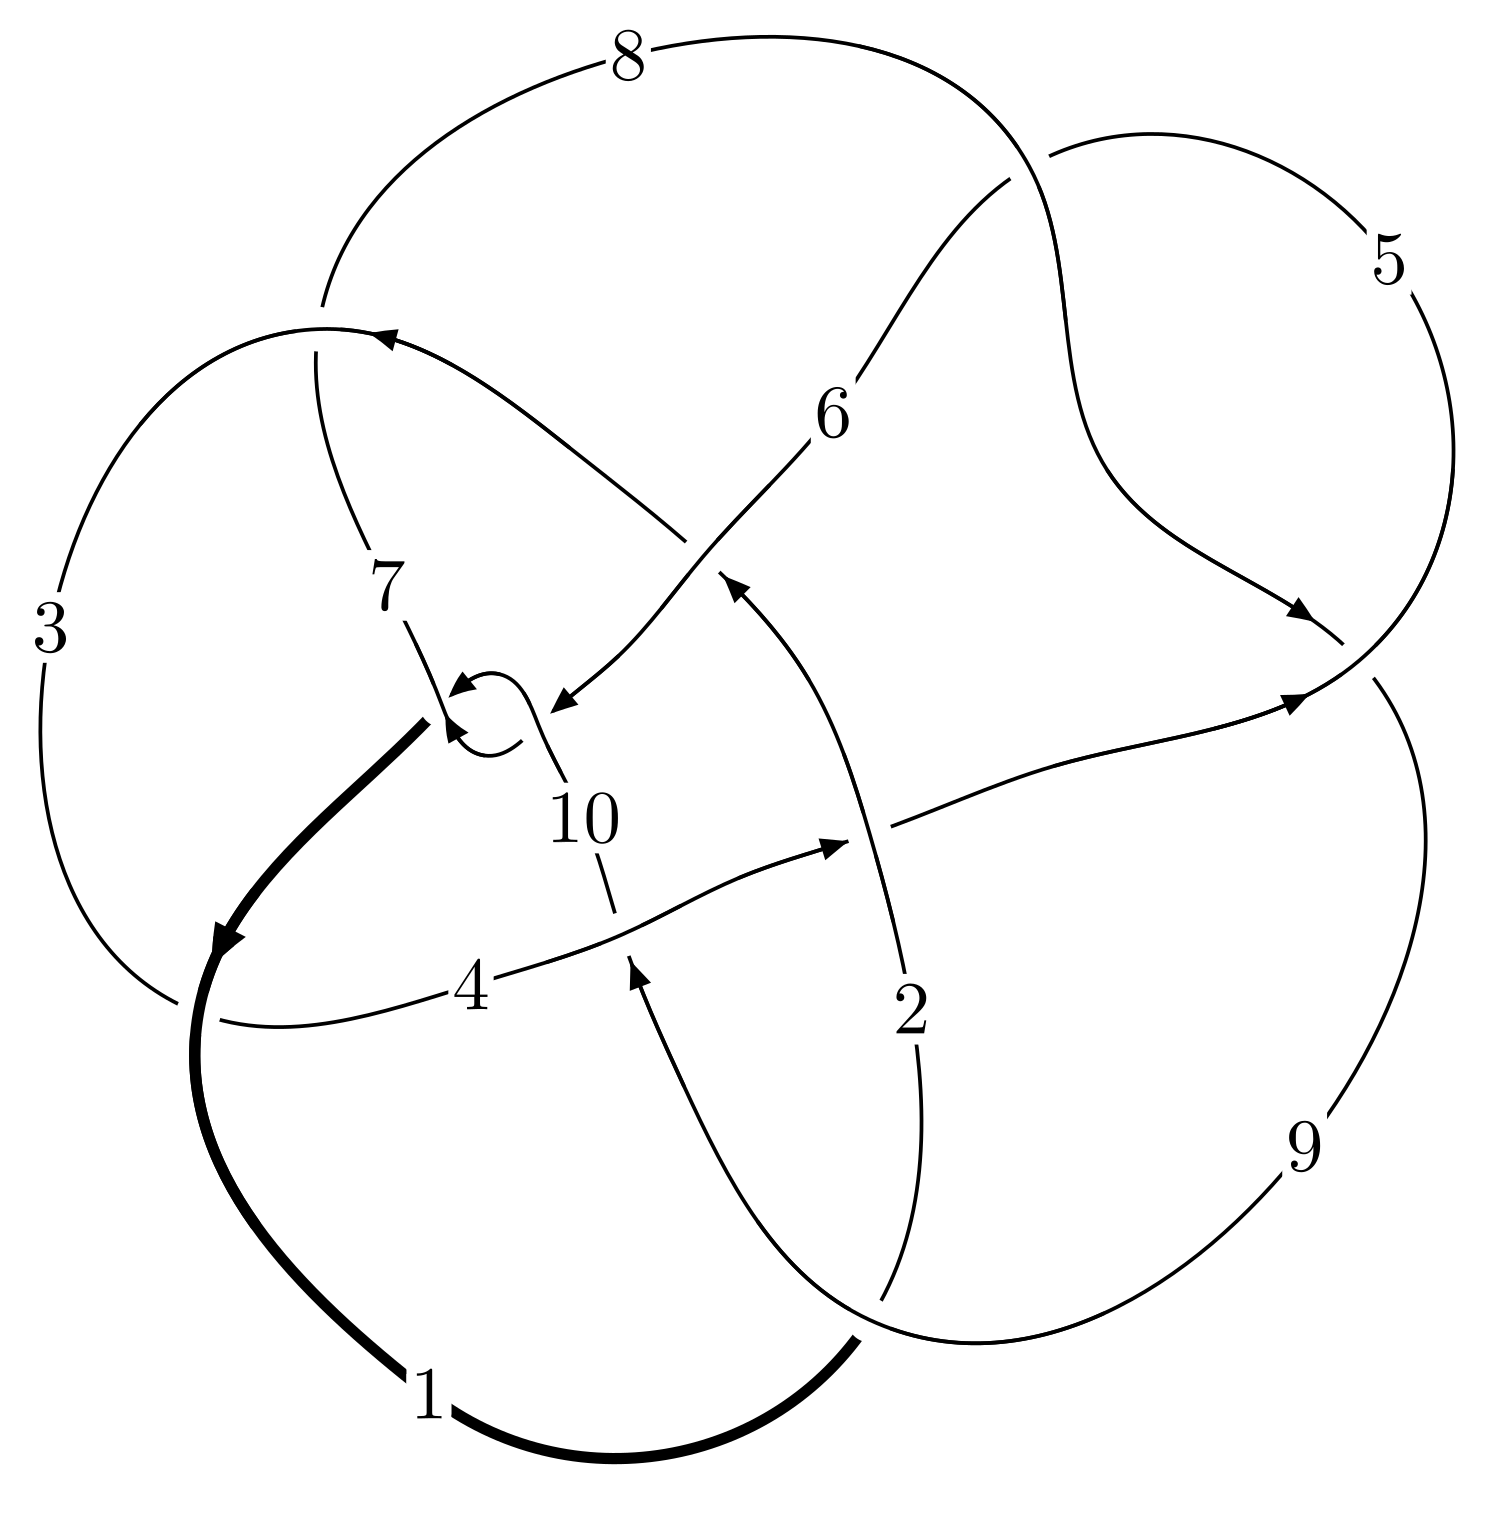
\includegraphics[width=112pt]{../../../GIT/diagram.site/Diagrams/png/203_10_119.png}\\
\ \ \ A knot diagram\footnotemark}&
\allowdisplaybreaks
\textbf{Linearized knot diagam} \\
\cline{2-2}
 &
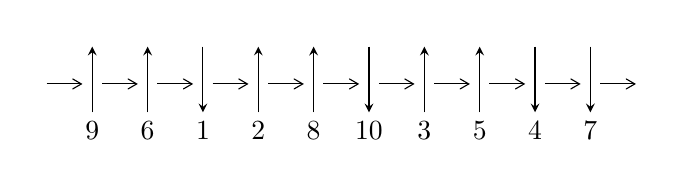
\begin{tikzpicture}[x=20pt, y=17pt]
	% nodes
	\node (C0) at (0, 0) {};
	\node (C1) at (1, 0) {};
	\node (C1U) at (1, +1) {};
	\node (C1D) at (1, -1) {9};

	\node (C2) at (2, 0) {};
	\node (C2U) at (2, +1) {};
	\node (C2D) at (2, -1) {6};

	\node (C3) at (3, 0) {};
	\node (C3U) at (3, +1) {};
	\node (C3D) at (3, -1) {1};

	\node (C4) at (4, 0) {};
	\node (C4U) at (4, +1) {};
	\node (C4D) at (4, -1) {2};

	\node (C5) at (5, 0) {};
	\node (C5U) at (5, +1) {};
	\node (C5D) at (5, -1) {8};

	\node (C6) at (6, 0) {};
	\node (C6U) at (6, +1) {};
	\node (C6D) at (6, -1) {10};

	\node (C7) at (7, 0) {};
	\node (C7U) at (7, +1) {};
	\node (C7D) at (7, -1) {3};

	\node (C8) at (8, 0) {};
	\node (C8U) at (8, +1) {};
	\node (C8D) at (8, -1) {5};

	\node (C9) at (9, 0) {};
	\node (C9U) at (9, +1) {};
	\node (C9D) at (9, -1) {4};

	\node (C10) at (10, 0) {};
	\node (C10U) at (10, +1) {};
	\node (C10D) at (10, -1) {7};
	\node (C11) at (11, 0) {};

	% arrows
	\draw[->,>={angle 60}]
	(C0) edge (C1) (C1) edge (C2) (C2) edge (C3) (C3) edge (C4) (C4) edge (C5) (C5) edge (C6) (C6) edge (C7) (C7) edge (C8) (C8) edge (C9) (C9) edge (C10) (C10) edge (C11) ;	\draw[->,>=stealth]
	(C1D) edge (C1U) (C2D) edge (C2U) (C3U) edge (C3D) (C4D) edge (C4U) (C5D) edge (C5U) (C6U) edge (C6D) (C7D) edge (C7U) (C8D) edge (C8U) (C9U) edge (C9D) (C10U) edge (C10D) ;
	\end{tikzpicture} \\
\hhline{~~} \\& 
\textbf{Solving Sequence} \\ \cline{2-2} 
 &
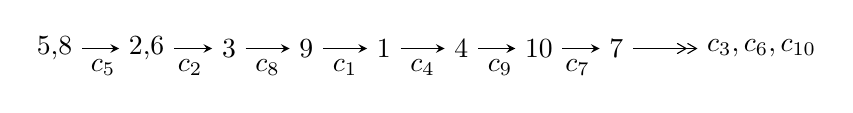
\begin{tikzpicture}[x=28pt, y=7pt]
	% node
	\node (A0) at (-1/8, 0) {5,8};
	\node (A1) at (17/16, 0) {2,6};
	\node (A2) at (17/8, 0) {3};
	\node (A3) at (25/8, 0) {9};
	\node (A4) at (33/8, 0) {1};
	\node (A5) at (41/8, 0) {4};
	\node (A6) at (49/8, 0) {10};
	\node (A7) at (57/8, 0) {7};
	\node (C1) at (1/2, -1) {$c_{5}$};
	\node (C2) at (13/8, -1) {$c_{2}$};
	\node (C3) at (21/8, -1) {$c_{8}$};
	\node (C4) at (29/8, -1) {$c_{1}$};
	\node (C5) at (37/8, -1) {$c_{4}$};
	\node (C6) at (45/8, -1) {$c_{9}$};
	\node (C7) at (53/8, -1) {$c_{7}$};
	\node (A8) at (9, 0) {$c_{3},c_{6},c_{10}$};

	% edge
	\draw[->,>=stealth]	
	(A0) edge (A1) (A1) edge (A2) (A2) edge (A3) (A3) edge (A4) (A4) edge (A5) (A5) edge (A6) (A6) edge (A7) ;
	\draw[->>,>={angle 60}]	
	(A7) edge (A8);
\end{tikzpicture} \\ 

\end{tabular} \\

\footnotetext{
The image of knot diagram is generated by the software ``\textbf{Draw programme}" developed by Andrew Bartholomew(\url{http://www.layer8.co.uk/maths/draw/index.htm\#Running-draw}), where we modified some parts for our purpose(\url{https://github.com/CATsTAILs/LinksPainter}).
}\phantom \\ \newline 
\centering \textbf{Ideals for irreducible components\footnotemark of $X_{\text{par}}$} 
 
\begin{align*}
I^u_{1}&=\langle 
3.28777\times10^{89} u^{59}-1.22268\times10^{90} u^{58}+\cdots+1.16518\times10^{90} b-4.76698\times10^{90},\\
\phantom{I^u_{1}}&\phantom{= \langle  }4.99619\times10^{90} u^{59}-1.95056\times10^{91} u^{58}+\cdots+1.16518\times10^{90} a-4.95274\times10^{91},\;u^{60}-4 u^{59}+\cdots-23 u+1\rangle \\
I^u_{2}&=\langle 
- u^9-4 u^7-2 u^6-7 u^5-5 u^4-7 u^3-5 u^2+b-4 u-2,\;u^7- u^6+3 u^5-2 u^4+2 u^3-3 u^2+a- u-2,\\
\phantom{I^u_{2}}&\phantom{= \langle  }u^{10}+u^9+5 u^8+6 u^7+12 u^6+13 u^5+15 u^4+12 u^3+9 u^2+4 u+1\rangle \\
\\
\end{align*}
\raggedright * 2 irreducible components of $\dim_{\mathbb{C}}=0$, with total 70 representations.\\
\footnotetext{All coefficients of polynomials are rational numbers. But the coefficients are sometimes approximated in decimal forms when there is not enough margin.}
\newpage
\renewcommand{\arraystretch}{1}
\centering \section*{I. $I^u_{1}= \langle 3.29\times10^{89} u^{59}-1.22\times10^{90} u^{58}+\cdots+1.17\times10^{90} b-4.77\times10^{90},\;5.00\times10^{90} u^{59}-1.95\times10^{91} u^{58}+\cdots+1.17\times10^{90} a-4.95\times10^{91},\;u^{60}-4 u^{59}+\cdots-23 u+1 \rangle$}
\flushleft \textbf{(i) Arc colorings}\\
\begin{tabular}{m{7pt} m{180pt} m{7pt} m{180pt} }
\flushright $a_{5}=$&$\begin{pmatrix}1\\0\end{pmatrix}$ \\
\flushright $a_{8}=$&$\begin{pmatrix}0\\u\end{pmatrix}$ \\
\flushright $a_{2}=$&$\begin{pmatrix}-4.28792 u^{59}+16.7404 u^{58}+\cdots-632.741 u+42.5063\\-0.282169 u^{59}+1.04935 u^{58}+\cdots-68.4354 u+4.09120\end{pmatrix}$ \\
\flushright $a_{6}=$&$\begin{pmatrix}1\\- u^2\end{pmatrix}$ \\
\flushright $a_{3}=$&$\begin{pmatrix}-4.49942 u^{59}+17.6872 u^{58}+\cdots-706.347 u+47.0087\\0.0395616 u^{59}-0.121304 u^{58}+\cdots-70.9634 u+4.19192\end{pmatrix}$ \\
\flushright $a_{9}=$&$\begin{pmatrix}u\\u\end{pmatrix}$ \\
\flushright $a_{1}=$&$\begin{pmatrix}-3.94168 u^{59}+15.4635 u^{58}+\cdots-636.369 u+42.8382\\0.0640690 u^{59}-0.227607 u^{58}+\cdots-72.0633 u+4.42310\end{pmatrix}$ \\
\flushright $a_{4}=$&$\begin{pmatrix}-1.42367 u^{59}+5.54425 u^{58}+\cdots-88.6243 u-5.93639\\0.806409 u^{59}-2.71615 u^{58}+\cdots+23.9853 u-2.83163\end{pmatrix}$ \\
\flushright $a_{10}=$&$\begin{pmatrix}-3.87666 u^{59}+15.1780 u^{58}+\cdots-470.845 u+20.7208\\-0.0321931 u^{59}+0.119215 u^{58}+\cdots-17.1665 u-0.190875\end{pmatrix}$ \\
\flushright $a_{7}=$&$\begin{pmatrix}5.78866 u^{59}-22.0859 u^{58}+\cdots+760.341 u-39.0347\\0.216555 u^{59}-0.514676 u^{58}+\cdots+42.0890 u-1.34596\end{pmatrix}$\\&\end{tabular}
\flushleft \textbf{(ii) Obstruction class $= -1$}\\~\\
\flushleft \textbf{(iii) Cusp Shapes $= 1.42721 u^{59}-4.42637 u^{58}+\cdots+298.469 u-20.6166$}\\~\\
\newpage\renewcommand{\arraystretch}{1}
\flushleft \textbf{(iv) u-Polynomials at the component}\newline \\
\begin{tabular}{m{50pt}|m{274pt}}
Crossings & \hspace{64pt}u-Polynomials at each crossing \\
\hline $$\begin{aligned}c_{1}\end{aligned}$$&$\begin{aligned}
&u^{60}+6 u^{59}+\cdots+543 u+79
\end{aligned}$\\
\hline $$\begin{aligned}c_{2}\end{aligned}$$&$\begin{aligned}
&u^{60}+u^{59}+\cdots+314 u+71
\end{aligned}$\\
\hline $$\begin{aligned}c_{3}\end{aligned}$$&$\begin{aligned}
&u^{60}+4 u^{59}+\cdots-90 u+31
\end{aligned}$\\
\hline $$\begin{aligned}c_{4}\end{aligned}$$&$\begin{aligned}
&u^{60}+4 u^{58}+\cdots+28 u+3
\end{aligned}$\\
\hline $$\begin{aligned}c_{5},c_{8}\end{aligned}$$&$\begin{aligned}
&u^{60}+4 u^{59}+\cdots+23 u+1
\end{aligned}$\\
\hline $$\begin{aligned}c_{6},c_{10}\end{aligned}$$&$\begin{aligned}
&u^{60}+2 u^{59}+\cdots+21 u+13
\end{aligned}$\\
\hline $$\begin{aligned}c_{7}\end{aligned}$$&$\begin{aligned}
&u^{60}+u^{59}+\cdots+1880 u+667
\end{aligned}$\\
\hline $$\begin{aligned}c_{9}\end{aligned}$$&$\begin{aligned}
&u^{60}+u^{59}+\cdots-22 u+1
\end{aligned}$\\
\hline
\end{tabular}\\~\\
\newpage\renewcommand{\arraystretch}{1}
\flushleft \textbf{(v) Riley Polynomials at the component}\newline \\
\begin{tabular}{m{50pt}|m{274pt}}
Crossings & \hspace{64pt}Riley Polynomials at each crossing \\
\hline $$\begin{aligned}c_{1}\end{aligned}$$&$\begin{aligned}
&y^{60}+14 y^{59}+\cdots+122113 y+6241
\end{aligned}$\\
\hline $$\begin{aligned}c_{2}\end{aligned}$$&$\begin{aligned}
&y^{60}+13 y^{59}+\cdots+80466 y+5041
\end{aligned}$\\
\hline $$\begin{aligned}c_{3}\end{aligned}$$&$\begin{aligned}
&y^{60}-16 y^{59}+\cdots-65698 y+961
\end{aligned}$\\
\hline $$\begin{aligned}c_{4}\end{aligned}$$&$\begin{aligned}
&y^{60}+8 y^{59}+\cdots+152 y+9
\end{aligned}$\\
\hline $$\begin{aligned}c_{5},c_{8}\end{aligned}$$&$\begin{aligned}
&y^{60}+46 y^{59}+\cdots-77 y+1
\end{aligned}$\\
\hline $$\begin{aligned}c_{6},c_{10}\end{aligned}$$&$\begin{aligned}
&y^{60}-36 y^{59}+\cdots-2183 y+169
\end{aligned}$\\
\hline $$\begin{aligned}c_{7}\end{aligned}$$&$\begin{aligned}
&y^{60}+21 y^{59}+\cdots+11382388 y+444889
\end{aligned}$\\
\hline $$\begin{aligned}c_{9}\end{aligned}$$&$\begin{aligned}
&y^{60}+5 y^{59}+\cdots-22 y+1
\end{aligned}$\\
\hline
\end{tabular}\\~\\
\newpage\flushleft \textbf{(vi) Complex Volumes and Cusp Shapes}
$$\begin{array}{c|c|c}  
\text{Solutions to }I^u_{1}& \I (\text{vol} + \sqrt{-1}CS) & \text{Cusp shape}\\
 \hline 
\begin{aligned}
u &= -0.623835 + 0.811166 I \\
a &= \phantom{-}0.859875 + 0.355902 I \\
b &= -0.636544 + 0.230444 I\end{aligned}
 & \phantom{-}0.77022 - 2.47923 I & \phantom{-0.000000 } 0. - 8.23551 I \\ \hline\begin{aligned}
u &= -0.623835 - 0.811166 I \\
a &= \phantom{-}0.859875 - 0.355902 I \\
b &= -0.636544 - 0.230444 I\end{aligned}
 & \phantom{-}0.77022 + 2.47923 I & \phantom{-0.000000 -}0. + 8.23551 I \\ \hline\begin{aligned}
u &= -0.390191 + 0.895254 I \\
a &= \phantom{-}0.454903 + 1.198220 I \\
b &= -0.222891 + 0.173390 I\end{aligned}
 & \phantom{-}0.48057 - 1.96275 I & \phantom{-}6.28895 + 2.92214 I \\ \hline\begin{aligned}
u &= -0.390191 - 0.895254 I \\
a &= \phantom{-}0.454903 - 1.198220 I \\
b &= -0.222891 - 0.173390 I\end{aligned}
 & \phantom{-}0.48057 + 1.96275 I & \phantom{-}6.28895 - 2.92214 I \\ \hline\begin{aligned}
u &= -0.057890 + 0.957459 I \\
a &= \phantom{-}0.90207 - 1.34370 I \\
b &= \phantom{-}0.307590 - 0.697419 I\end{aligned}
 & -1.69174 - 2.07365 I & -0.35018 + 3.75765 I \\ \hline\begin{aligned}
u &= -0.057890 - 0.957459 I \\
a &= \phantom{-}0.90207 + 1.34370 I \\
b &= \phantom{-}0.307590 + 0.697419 I\end{aligned}
 & -1.69174 + 2.07365 I & -0.35018 - 3.75765 I \\ \hline\begin{aligned}
u &= \phantom{-}0.055199 + 1.062610 I \\
a &= -0.240418 + 0.784604 I \\
b &= \phantom{-}1.238390 + 0.475118 I\end{aligned}
 & -1.53778 + 2.56920 I & \phantom{-0.000000 } 0 \\ \hline\begin{aligned}
u &= \phantom{-}0.055199 - 1.062610 I \\
a &= -0.240418 - 0.784604 I \\
b &= \phantom{-}1.238390 - 0.475118 I\end{aligned}
 & -1.53778 - 2.56920 I & \phantom{-0.000000 } 0 \\ \hline\begin{aligned}
u &= \phantom{-}1.098360 + 0.127961 I \\
a &= \phantom{-}0.283818 - 0.122637 I \\
b &= -0.223247 - 0.733150 I\end{aligned}
 & -4.15031 - 0.75171 I & \phantom{-0.000000 } 0 \\ \hline\begin{aligned}
u &= \phantom{-}1.098360 - 0.127961 I \\
a &= \phantom{-}0.283818 + 0.122637 I \\
b &= -0.223247 + 0.733150 I\end{aligned}
 & -4.15031 + 0.75171 I & \phantom{-0.000000 } 0\\
 \hline 
 \end{array}$$\newpage$$\begin{array}{c|c|c}  
\text{Solutions to }I^u_{1}& \I (\text{vol} + \sqrt{-1}CS) & \text{Cusp shape}\\
 \hline 
\begin{aligned}
u &= \phantom{-}0.252033 + 1.079010 I \\
a &= \phantom{-}0.09965 + 1.68364 I \\
b &= \phantom{-}1.16552 + 1.29014 I\end{aligned}
 & -1.42019 + 3.81670 I & \phantom{-0.000000 } 0 \\ \hline\begin{aligned}
u &= \phantom{-}0.252033 - 1.079010 I \\
a &= \phantom{-}0.09965 - 1.68364 I \\
b &= \phantom{-}1.16552 - 1.29014 I\end{aligned}
 & -1.42019 - 3.81670 I & \phantom{-0.000000 } 0 \\ \hline\begin{aligned}
u &= -0.790615 + 0.388915 I \\
a &= \phantom{-}0.890087 - 0.241883 I \\
b &= \phantom{-}0.796474 + 0.786684 I\end{aligned}
 & -0.44456 + 2.32036 I & -1.97518 - 4.64341 I \\ \hline\begin{aligned}
u &= -0.790615 - 0.388915 I \\
a &= \phantom{-}0.890087 + 0.241883 I \\
b &= \phantom{-}0.796474 - 0.786684 I\end{aligned}
 & -0.44456 - 2.32036 I & -1.97518 + 4.64341 I \\ \hline\begin{aligned}
u &= \phantom{-}0.303509 + 1.104720 I \\
a &= -0.22498 - 2.03796 I \\
b &= -0.308920 - 0.321579 I\end{aligned}
 & -4.17954 + 7.17743 I & \phantom{-0.000000 } 0 \\ \hline\begin{aligned}
u &= \phantom{-}0.303509 - 1.104720 I \\
a &= -0.22498 + 2.03796 I \\
b &= -0.308920 + 0.321579 I\end{aligned}
 & -4.17954 - 7.17743 I & \phantom{-0.000000 } 0 \\ \hline\begin{aligned}
u &= \phantom{-}1.140370 + 0.172582 I \\
a &= -0.0216976 - 0.0536118 I \\
b &= -0.860595 - 0.757350 I\end{aligned}
 & -1.92721 + 10.19580 I & \phantom{-0.000000 } 0 \\ \hline\begin{aligned}
u &= \phantom{-}1.140370 - 0.172582 I \\
a &= -0.0216976 + 0.0536118 I \\
b &= -0.860595 + 0.757350 I\end{aligned}
 & -1.92721 - 10.19580 I & \phantom{-0.000000 } 0 \\ \hline\begin{aligned}
u &= -0.423700 + 1.097000 I \\
a &= \phantom{-}0.01484 - 1.74876 I \\
b &= \phantom{-}0.98126 - 1.54901 I\end{aligned}
 & -2.67312 - 6.89147 I & \phantom{-0.000000 } 0 \\ \hline\begin{aligned}
u &= -0.423700 - 1.097000 I \\
a &= \phantom{-}0.01484 + 1.74876 I \\
b &= \phantom{-}0.98126 + 1.54901 I\end{aligned}
 & -2.67312 + 6.89147 I & \phantom{-0.000000 } 0\\
 \hline 
 \end{array}$$\newpage$$\begin{array}{c|c|c}  
\text{Solutions to }I^u_{1}& \I (\text{vol} + \sqrt{-1}CS) & \text{Cusp shape}\\
 \hline 
\begin{aligned}
u &= -1.173550 + 0.196304 I \\
a &= \phantom{-}0.1089490 + 0.0035265 I \\
b &= -0.723525 + 0.554514 I\end{aligned}
 & \phantom{-}1.66896 - 4.09599 I & \phantom{-0.000000 } 0 \\ \hline\begin{aligned}
u &= -1.173550 - 0.196304 I \\
a &= \phantom{-}0.1089490 - 0.0035265 I \\
b &= -0.723525 - 0.554514 I\end{aligned}
 & \phantom{-}1.66896 + 4.09599 I & \phantom{-0.000000 } 0 \\ \hline\begin{aligned}
u &= \phantom{-}0.105236 + 1.199410 I \\
a &= -0.79780 + 1.85890 I \\
b &= -1.31875 + 1.79980 I\end{aligned}
 & -6.90749 + 6.01393 I & \phantom{-0.000000 } 0 \\ \hline\begin{aligned}
u &= \phantom{-}0.105236 - 1.199410 I \\
a &= -0.79780 - 1.85890 I \\
b &= -1.31875 - 1.79980 I\end{aligned}
 & -6.90749 - 6.01393 I & \phantom{-0.000000 } 0 \\ \hline\begin{aligned}
u &= -0.057124 + 1.206740 I \\
a &= -0.225137 - 1.384350 I \\
b &= -0.83604 - 1.24262 I\end{aligned}
 & -3.96912 - 1.82451 I & \phantom{-0.000000 } 0 \\ \hline\begin{aligned}
u &= -0.057124 - 1.206740 I \\
a &= -0.225137 + 1.384350 I \\
b &= -0.83604 + 1.24262 I\end{aligned}
 & -3.96912 + 1.82451 I & \phantom{-0.000000 } 0 \\ \hline\begin{aligned}
u &= -0.057398 + 1.224090 I \\
a &= -0.66515 - 1.99713 I \\
b &= \phantom{-}0.539561 - 0.979683 I\end{aligned}
 & -7.31597 - 5.19158 I & \phantom{-0.000000 } 0 \\ \hline\begin{aligned}
u &= -0.057398 - 1.224090 I \\
a &= -0.66515 + 1.99713 I \\
b &= \phantom{-}0.539561 + 0.979683 I\end{aligned}
 & -7.31597 + 5.19158 I & \phantom{-0.000000 } 0 \\ \hline\begin{aligned}
u &= \phantom{-}0.539940 + 0.503116 I \\
a &= \phantom{-}1.024080 + 0.843151 I \\
b &= \phantom{-}0.880526 - 0.425648 I\end{aligned}
 & \phantom{-}0.285692 - 0.756946 I & \phantom{-}1.15945 - 1.79896 I \\ \hline\begin{aligned}
u &= \phantom{-}0.539940 - 0.503116 I \\
a &= \phantom{-}1.024080 - 0.843151 I \\
b &= \phantom{-}0.880526 + 0.425648 I\end{aligned}
 & \phantom{-}0.285692 + 0.756946 I & \phantom{-}1.15945 + 1.79896 I\\
 \hline 
 \end{array}$$\newpage$$\begin{array}{c|c|c}  
\text{Solutions to }I^u_{1}& \I (\text{vol} + \sqrt{-1}CS) & \text{Cusp shape}\\
 \hline 
\begin{aligned}
u &= -0.696757 + 0.013245 I \\
a &= \phantom{-}0.218959 - 0.031077 I \\
b &= \phantom{-}0.950374 + 0.230216 I\end{aligned}
 & \phantom{-}1.77833 + 0.12398 I & \phantom{-}7.12326 + 1.43443 I \\ \hline\begin{aligned}
u &= -0.696757 - 0.013245 I \\
a &= \phantom{-}0.218959 + 0.031077 I \\
b &= \phantom{-}0.950374 - 0.230216 I\end{aligned}
 & \phantom{-}1.77833 - 0.12398 I & \phantom{-}7.12326 - 1.43443 I \\ \hline\begin{aligned}
u &= \phantom{-}0.262291 + 1.287330 I \\
a &= \phantom{-}0.29769 + 2.09008 I \\
b &= \phantom{-}0.97062 + 1.39698 I\end{aligned}
 & -3.13949 + 6.16052 I & \phantom{-0.000000 } 0 \\ \hline\begin{aligned}
u &= \phantom{-}0.262291 - 1.287330 I \\
a &= \phantom{-}0.29769 - 2.09008 I \\
b &= \phantom{-}0.97062 - 1.39698 I\end{aligned}
 & -3.13949 - 6.16052 I & \phantom{-0.000000 } 0 \\ \hline\begin{aligned}
u &= \phantom{-}0.097078 + 1.316500 I \\
a &= -0.859018 + 0.495607 I \\
b &= -1.55967 + 0.51228 I\end{aligned}
 & -6.87032 - 1.61985 I & \phantom{-0.000000 } 0 \\ \hline\begin{aligned}
u &= \phantom{-}0.097078 - 1.316500 I \\
a &= -0.859018 - 0.495607 I \\
b &= -1.55967 - 0.51228 I\end{aligned}
 & -6.87032 + 1.61985 I & \phantom{-0.000000 } 0 \\ \hline\begin{aligned}
u &= -0.313462 + 1.288310 I \\
a &= \phantom{-}0.49264 - 1.63832 I \\
b &= \phantom{-}1.01214 - 1.22490 I\end{aligned}
 & -2.23892 - 3.83057 I & \phantom{-0.000000 } 0 \\ \hline\begin{aligned}
u &= -0.313462 - 1.288310 I \\
a &= \phantom{-}0.49264 + 1.63832 I \\
b &= \phantom{-}1.01214 + 1.22490 I\end{aligned}
 & -2.23892 + 3.83057 I & \phantom{-0.000000 } 0 \\ \hline\begin{aligned}
u &= \phantom{-}0.588701 + 0.273361 I \\
a &= \phantom{-}1.06281 + 0.93632 I \\
b &= -0.866958 + 0.207225 I\end{aligned}
 & -1.77283 - 3.70444 I & \phantom{-}2.15456 + 4.83060 I \\ \hline\begin{aligned}
u &= \phantom{-}0.588701 - 0.273361 I \\
a &= \phantom{-}1.06281 - 0.93632 I \\
b &= -0.866958 - 0.207225 I\end{aligned}
 & -1.77283 + 3.70444 I & \phantom{-}2.15456 - 4.83060 I\\
 \hline 
 \end{array}$$\newpage$$\begin{array}{c|c|c}  
\text{Solutions to }I^u_{1}& \I (\text{vol} + \sqrt{-1}CS) & \text{Cusp shape}\\
 \hline 
\begin{aligned}
u &= -0.073825 + 1.367230 I \\
a &= \phantom{-}0.802201 + 0.446279 I \\
b &= -0.161175 + 0.349105 I\end{aligned}
 & -6.64861 - 0.13946 I & \phantom{-0.000000 } 0 \\ \hline\begin{aligned}
u &= -0.073825 - 1.367230 I \\
a &= \phantom{-}0.802201 - 0.446279 I \\
b &= -0.161175 - 0.349105 I\end{aligned}
 & -6.64861 + 0.13946 I & \phantom{-0.000000 } 0 \\ \hline\begin{aligned}
u &= \phantom{-}0.540634 + 0.052002 I \\
a &= -0.358037 + 0.018404 I \\
b &= \phantom{-}0.990107 + 0.775650 I\end{aligned}
 & \phantom{-}1.01358 + 3.09322 I & \phantom{-}5.20661 - 7.95930 I \\ \hline\begin{aligned}
u &= \phantom{-}0.540634 - 0.052002 I \\
a &= -0.358037 - 0.018404 I \\
b &= \phantom{-}0.990107 - 0.775650 I\end{aligned}
 & \phantom{-}1.01358 - 3.09322 I & \phantom{-}5.20661 + 7.95930 I \\ \hline\begin{aligned}
u &= \phantom{-}0.48204 + 1.37578 I \\
a &= \phantom{-}0.289297 - 1.243460 I \\
b &= -0.783244 - 0.988185 I\end{aligned}
 & -8.85403 + 4.69065 I & \phantom{-0.000000 } 0 \\ \hline\begin{aligned}
u &= \phantom{-}0.48204 - 1.37578 I \\
a &= \phantom{-}0.289297 + 1.243460 I \\
b &= -0.783244 + 0.988185 I\end{aligned}
 & -8.85403 - 4.69065 I & \phantom{-0.000000 } 0 \\ \hline\begin{aligned}
u &= \phantom{-}0.56774 + 1.38515 I \\
a &= -0.309520 + 1.074330 I \\
b &= \phantom{-}0.299852 + 1.192800 I\end{aligned}
 & -8.17971 + 6.88009 I & \phantom{-0.000000 } 0 \\ \hline\begin{aligned}
u &= \phantom{-}0.56774 - 1.38515 I \\
a &= -0.309520 - 1.074330 I \\
b &= \phantom{-}0.299852 - 1.192800 I\end{aligned}
 & -8.17971 - 6.88009 I & \phantom{-0.000000 } 0 \\ \hline\begin{aligned}
u &= -0.50546 + 1.41839 I \\
a &= -0.069865 + 1.320870 I \\
b &= -1.10129 + 1.06163 I\end{aligned}
 & -3.32542 - 9.91193 I & \phantom{-0.000000 } 0 \\ \hline\begin{aligned}
u &= -0.50546 - 1.41839 I \\
a &= -0.069865 - 1.320870 I \\
b &= -1.10129 - 1.06163 I\end{aligned}
 & -3.32542 + 9.91193 I & \phantom{-0.000000 } 0\\
 \hline 
 \end{array}$$\newpage$$\begin{array}{c|c|c}  
\text{Solutions to }I^u_{1}& \I (\text{vol} + \sqrt{-1}CS) & \text{Cusp shape}\\
 \hline 
\begin{aligned}
u &= \phantom{-}0.49893 + 1.42456 I \\
a &= -0.12004 - 1.52962 I \\
b &= -1.14876 - 1.24339 I\end{aligned}
 & -6.9242 + 15.9387 I & \phantom{-0.000000 } 0 \\ \hline\begin{aligned}
u &= \phantom{-}0.49893 - 1.42456 I \\
a &= -0.12004 + 1.52962 I \\
b &= -1.14876 + 1.24339 I\end{aligned}
 & -6.9242 - 15.9387 I & \phantom{-0.000000 } 0 \\ \hline\begin{aligned}
u &= -0.39076 + 1.51085 I \\
a &= \phantom{-}0.232798 - 0.759750 I \\
b &= \phantom{-}0.621503 - 0.751780 I\end{aligned}
 & -3.26872 - 3.24397 I & \phantom{-0.000000 } 0 \\ \hline\begin{aligned}
u &= -0.39076 - 1.51085 I \\
a &= \phantom{-}0.232798 + 0.759750 I \\
b &= \phantom{-}0.621503 + 0.751780 I\end{aligned}
 & -3.26872 + 3.24397 I & \phantom{-0.000000 } 0 \\ \hline\begin{aligned}
u &= \phantom{-}0.105930 + 0.285642 I \\
a &= \phantom{-}1.73848 + 2.14934 I \\
b &= \phantom{-}0.223189 - 0.473560 I\end{aligned}
 & \phantom{-}0.08914 - 1.52136 I & \phantom{-}0.92288 + 3.10853 I \\ \hline\begin{aligned}
u &= \phantom{-}0.105930 - 0.285642 I \\
a &= \phantom{-}1.73848 - 2.14934 I \\
b &= \phantom{-}0.223189 + 0.473560 I\end{aligned}
 & \phantom{-}0.08914 + 1.52136 I & \phantom{-}0.92288 - 3.10853 I \\ \hline\begin{aligned}
u &= \phantom{-}0.81740 + 1.64815 I \\
a &= -0.236080 + 0.190955 I \\
b &= -0.000901 + 0.445406 I\end{aligned}
 & -5.53864 - 3.01539 I & \phantom{-0.000000 } 0 \\ \hline\begin{aligned}
u &= \phantom{-}0.81740 - 1.64815 I \\
a &= -0.236080 - 0.190955 I \\
b &= -0.000901 - 0.445406 I\end{aligned}
 & -5.53864 + 3.01539 I & \phantom{-0.000000 } 0 \\ \hline\begin{aligned}
u &= \phantom{-}0.0991795 + 0.0504499 I \\
a &= \phantom{-}2.85459 - 9.86759 I \\
b &= -0.224592 - 1.103140 I\end{aligned}
 & -3.57991 - 4.96662 I & -0.78194 + 5.62106 I \\ \hline\begin{aligned}
u &= \phantom{-}0.0991795 - 0.0504499 I \\
a &= \phantom{-}2.85459 + 9.86759 I \\
b &= -0.224592 + 1.103140 I\end{aligned}
 & -3.57991 + 4.96662 I & -0.78194 - 5.62106 I\\
 \hline 
 \end{array}$$\newpage\newpage\renewcommand{\arraystretch}{1}
\centering \section*{II. $I^u_{2}= \langle - u^9-4 u^7+\cdots+b-2,\;u^7- u^6+3 u^5-2 u^4+2 u^3-3 u^2+a- u-2,\;u^{10}+u^9+\cdots+4 u+1 \rangle$}
\flushleft \textbf{(i) Arc colorings}\\
\begin{tabular}{m{7pt} m{180pt} m{7pt} m{180pt} }
\flushright $a_{5}=$&$\begin{pmatrix}1\\0\end{pmatrix}$ \\
\flushright $a_{8}=$&$\begin{pmatrix}0\\u\end{pmatrix}$ \\
\flushright $a_{2}=$&$\begin{pmatrix}- u^7+u^6-3 u^5+2 u^4-2 u^3+3 u^2+u+2\\u^9+4 u^7+2 u^6+7 u^5+5 u^4+7 u^3+5 u^2+4 u+2\end{pmatrix}$ \\
\flushright $a_{6}=$&$\begin{pmatrix}1\\- u^2\end{pmatrix}$ \\
\flushright $a_{3}=$&$\begin{pmatrix}u^8+5 u^6+2 u^5+10 u^4+6 u^3+10 u^2+5 u+4\\u^9+u^8+5 u^7+6 u^6+12 u^5+13 u^4+15 u^3+12 u^2+8 u+3\end{pmatrix}$ \\
\flushright $a_{9}=$&$\begin{pmatrix}u\\u\end{pmatrix}$ \\
\flushright $a_{1}=$&$\begin{pmatrix}- u^9-5 u^7- u^6-10 u^5-3 u^4-8 u^3-2 u^2-2 u+1\\u^3+u+1\end{pmatrix}$ \\
\flushright $a_{4}=$&$\begin{pmatrix}u^9+2 u^8+5 u^7+11 u^6+14 u^5+22 u^4+20 u^3+20 u^2+11 u+6\\2 u^9+u^8+9 u^7+8 u^6+19 u^5+17 u^4+21 u^3+15 u^2+10 u+3\end{pmatrix}$ \\
\flushright $a_{10}=$&$\begin{pmatrix}-3 u^9- u^8-15 u^7-9 u^6-32 u^5-22 u^4-33 u^3-19 u^2-15 u-2\\u^9+u^8+4 u^7+6 u^6+8 u^5+11 u^4+9 u^3+8 u^2+5 u+3\end{pmatrix}$ \\
\flushright $a_{7}=$&$\begin{pmatrix}-3 u^9- u^8-13 u^7-8 u^6-25 u^5-16 u^4-23 u^3-11 u^2-10 u-1\\u^8+u^7+5 u^6+5 u^5+11 u^4+9 u^3+10 u^2+6 u+3\end{pmatrix}$\\&\end{tabular}
\flushleft \textbf{(ii) Obstruction class $= 1$}\\~\\
\flushleft \textbf{(iii) Cusp Shapes $= -10 u^9+3 u^8-39 u^7-3 u^6-57 u^5-14 u^4-31 u^3-8 u^2-7 u+6$}\\~\\
\newpage\renewcommand{\arraystretch}{1}
\flushleft \textbf{(iv) u-Polynomials at the component}\newline \\
\begin{tabular}{m{50pt}|m{274pt}}
Crossings & \hspace{64pt}u-Polynomials at each crossing \\
\hline $$\begin{aligned}c_{1}\end{aligned}$$&$\begin{aligned}
&u^{10}- u^9+u^8+3 u^7+4 u^4+2 u^2+1
\end{aligned}$\\
\hline $$\begin{aligned}c_{2}\end{aligned}$$&$\begin{aligned}
&u^{10}+2 u^8+4 u^7+2 u^6+3 u^5+6 u^4+4 u^3+u^2+u+1
\end{aligned}$\\
\hline $$\begin{aligned}c_{3}\end{aligned}$$&$\begin{aligned}
&u^{10}+5 u^9+\cdots+5 u+1
\end{aligned}$\\
\hline $$\begin{aligned}c_{4}\end{aligned}$$&$\begin{aligned}
&u^{10}-5 u^9+14 u^8-24 u^7+29 u^6-24 u^5+11 u^4+u^3-2 u^2- u+1
\end{aligned}$\\
\hline $$\begin{aligned}c_{5}\end{aligned}$$&$\begin{aligned}
&u^{10}+u^9+5 u^8+6 u^7+12 u^6+13 u^5+15 u^4+12 u^3+9 u^2+4 u+1
\end{aligned}$\\
\hline $$\begin{aligned}c_{6}\end{aligned}$$&$\begin{aligned}
&u^{10}- u^9-2 u^8+4 u^7-5 u^5+5 u^4+2 u^3-4 u^2+1
\end{aligned}$\\
\hline $$\begin{aligned}c_{7}\end{aligned}$$&$\begin{aligned}
&u^{10}+3 u^7+2 u^6+2 u^5+2 u^4+3 u^3+4 u^2+u+1
\end{aligned}$\\
\hline $$\begin{aligned}c_{8}\end{aligned}$$&$\begin{aligned}
&u^{10}- u^9+5 u^8-6 u^7+12 u^6-13 u^5+15 u^4-12 u^3+9 u^2-4 u+1
\end{aligned}$\\
\hline $$\begin{aligned}c_{9}\end{aligned}$$&$\begin{aligned}
&u^{10}+2 u^8+4 u^6+3 u^3+u^2- u+1
\end{aligned}$\\
\hline $$\begin{aligned}c_{10}\end{aligned}$$&$\begin{aligned}
&u^{10}+u^9-2 u^8-4 u^7+5 u^5+5 u^4-2 u^3-4 u^2+1
\end{aligned}$\\
\hline
\end{tabular}\\~\\
\newpage\renewcommand{\arraystretch}{1}
\flushleft \textbf{(v) Riley Polynomials at the component}\newline \\
\begin{tabular}{m{50pt}|m{274pt}}
Crossings & \hspace{64pt}Riley Polynomials at each crossing \\
\hline $$\begin{aligned}c_{1}\end{aligned}$$&$\begin{aligned}
&y^{10}+y^9+7 y^8- y^7+12 y^6+6 y^5+18 y^4+16 y^3+12 y^2+4 y+1
\end{aligned}$\\
\hline $$\begin{aligned}c_{2}\end{aligned}$$&$\begin{aligned}
&y^{10}+4 y^9+8 y^8+4 y^7+6 y^6-11 y^5+12 y^4-6 y^3+5 y^2+y+1
\end{aligned}$\\
\hline $$\begin{aligned}c_{3}\end{aligned}$$&$\begin{aligned}
&y^{10}+3 y^9+2 y^8-8 y^7-35 y^6+138 y^4+105 y^3+27 y^2+5 y+1
\end{aligned}$\\
\hline $$\begin{aligned}c_{4}\end{aligned}$$&$\begin{aligned}
&y^{10}+3 y^9+14 y^8+18 y^7+3 y^6+46 y^5+33 y^4-35 y^3+28 y^2-5 y+1
\end{aligned}$\\
\hline $$\begin{aligned}c_{5},c_{8}\end{aligned}$$&$\begin{aligned}
&y^{10}+9 y^9+\cdots+2 y+1
\end{aligned}$\\
\hline $$\begin{aligned}c_{6},c_{10}\end{aligned}$$&$\begin{aligned}
&y^{10}-5 y^9+\cdots-8 y+1
\end{aligned}$\\
\hline $$\begin{aligned}c_{7}\end{aligned}$$&$\begin{aligned}
&y^{10}+4 y^8-5 y^7-12 y^5+2 y^4+7 y^3+14 y^2+7 y+1
\end{aligned}$\\
\hline $$\begin{aligned}c_{9}\end{aligned}$$&$\begin{aligned}
&y^{10}+4 y^9+12 y^8+16 y^7+18 y^6+6 y^5+12 y^4- y^3+7 y^2+y+1
\end{aligned}$\\
\hline
\end{tabular}\\~\\
\newpage\flushleft \textbf{(vi) Complex Volumes and Cusp Shapes}
$$\begin{array}{c|c|c}  
\text{Solutions to }I^u_{2}& \I (\text{vol} + \sqrt{-1}CS) & \text{Cusp shape}\\
 \hline 
\begin{aligned}
u &= -0.569171 + 0.652818 I \\
a &= -1.156860 - 0.167161 I \\
b &= \phantom{-}0.666955 - 0.329661 I\end{aligned}
 & \phantom{-}0.80863 - 2.83685 I & \phantom{-}3.98230 + 13.24479 I \\ \hline\begin{aligned}
u &= -0.569171 - 0.652818 I \\
a &= -1.156860 + 0.167161 I \\
b &= \phantom{-}0.666955 + 0.329661 I\end{aligned}
 & \phantom{-}0.80863 + 2.83685 I & \phantom{-}3.98230 - 13.24479 I \\ \hline\begin{aligned}
u &= \phantom{-}0.257088 + 1.121830 I \\
a &= -0.53465 + 2.12743 I \\
b &= \phantom{-}0.069226 + 1.285130 I\end{aligned}
 & -5.27004 + 6.36836 I & -3.95341 - 6.63467 I \\ \hline\begin{aligned}
u &= \phantom{-}0.257088 - 1.121830 I \\
a &= -0.53465 - 2.12743 I \\
b &= \phantom{-}0.069226 - 1.285130 I\end{aligned}
 & -5.27004 - 6.36836 I & -3.95341 + 6.63467 I \\ \hline\begin{aligned}
u &= -0.265511 + 1.239090 I \\
a &= \phantom{-}0.42180 - 1.89279 I \\
b &= \phantom{-}1.14707 - 1.48128 I\end{aligned}
 & -2.50173 - 4.70796 I & -2.30544 + 6.58589 I \\ \hline\begin{aligned}
u &= -0.265511 - 1.239090 I \\
a &= \phantom{-}0.42180 + 1.89279 I \\
b &= \phantom{-}1.14707 + 1.48128 I\end{aligned}
 & -2.50173 + 4.70796 I & -2.30544 - 6.58589 I \\ \hline\begin{aligned}
u &= -0.409125 + 0.329081 I \\
a &= \phantom{-}1.37279 - 0.74482 I \\
b &= \phantom{-}1.006320 + 0.639149 I\end{aligned}
 & \phantom{-}0.60938 + 1.82644 I & \phantom{-}5.24506 - 2.77183 I \\ \hline\begin{aligned}
u &= -0.409125 - 0.329081 I \\
a &= \phantom{-}1.37279 + 0.74482 I \\
b &= \phantom{-}1.006320 - 0.639149 I\end{aligned}
 & \phantom{-}0.60938 - 1.82644 I & \phantom{-}5.24506 + 2.77183 I \\ \hline\begin{aligned}
u &= \phantom{-}0.48672 + 1.42706 I \\
a &= -0.1030920 + 0.0771624 I \\
b &= -0.389573 - 0.258635 I\end{aligned}
 & -5.16077 - 2.93340 I & \phantom{-}2.03148 + 3.30765 I \\ \hline\begin{aligned}
u &= \phantom{-}0.48672 - 1.42706 I \\
a &= -0.1030920 - 0.0771624 I \\
b &= -0.389573 + 0.258635 I\end{aligned}
 & -5.16077 + 2.93340 I & \phantom{-}2.03148 - 3.30765 I\\
 \hline 
 \end{array}$$\newpage
\newpage\renewcommand{\arraystretch}{1}
\centering \section*{ III. u-Polynomials}
\begin{tabular}{m{50pt}|m{274pt}}
Crossings & \hspace{64pt}u-Polynomials at each crossing \\
\hline $$\begin{aligned}c_{1}\end{aligned}$$&$\begin{aligned}
&(u^{10}- u^9+u^8+3 u^7+4 u^4+2 u^2+1)(u^{60}+6 u^{59}+\cdots+543 u+79)
\end{aligned}$\\
\hline $$\begin{aligned}c_{2}\end{aligned}$$&$\begin{aligned}
&(u^{10}+2 u^8+4 u^7+2 u^6+3 u^5+6 u^4+4 u^3+u^2+u+1)\\
&\cdot(u^{60}+u^{59}+\cdots+314 u+71)
\end{aligned}$\\
\hline $$\begin{aligned}c_{3}\end{aligned}$$&$\begin{aligned}
&(u^{10}+5 u^9+\cdots+5 u+1)(u^{60}+4 u^{59}+\cdots-90 u+31)
\end{aligned}$\\
\hline $$\begin{aligned}c_{4}\end{aligned}$$&$\begin{aligned}
&(u^{10}-5 u^9+14 u^8-24 u^7+29 u^6-24 u^5+11 u^4+u^3-2 u^2- u+1)\\
&\cdot(u^{60}+4 u^{58}+\cdots+28 u+3)
\end{aligned}$\\
\hline $$\begin{aligned}c_{5}\end{aligned}$$&$\begin{aligned}
&(u^{10}+u^9+5 u^8+6 u^7+12 u^6+13 u^5+15 u^4+12 u^3+9 u^2+4 u+1)\\
&\cdot(u^{60}+4 u^{59}+\cdots+23 u+1)
\end{aligned}$\\
\hline $$\begin{aligned}c_{6}\end{aligned}$$&$\begin{aligned}
&(u^{10}- u^9-2 u^8+4 u^7-5 u^5+5 u^4+2 u^3-4 u^2+1)\\
&\cdot(u^{60}+2 u^{59}+\cdots+21 u+13)
\end{aligned}$\\
\hline $$\begin{aligned}c_{7}\end{aligned}$$&$\begin{aligned}
&(u^{10}+3 u^7+2 u^6+2 u^5+2 u^4+3 u^3+4 u^2+u+1)\\
&\cdot(u^{60}+u^{59}+\cdots+1880 u+667)
\end{aligned}$\\
\hline $$\begin{aligned}c_{8}\end{aligned}$$&$\begin{aligned}
&(u^{10}- u^9+5 u^8-6 u^7+12 u^6-13 u^5+15 u^4-12 u^3+9 u^2-4 u+1)\\
&\cdot(u^{60}+4 u^{59}+\cdots+23 u+1)
\end{aligned}$\\
\hline $$\begin{aligned}c_{9}\end{aligned}$$&$\begin{aligned}
&(u^{10}+2 u^8+4 u^6+3 u^3+u^2- u+1)(u^{60}+u^{59}+\cdots-22 u+1)
\end{aligned}$\\
\hline $$\begin{aligned}c_{10}\end{aligned}$$&$\begin{aligned}
&(u^{10}+u^9-2 u^8-4 u^7+5 u^5+5 u^4-2 u^3-4 u^2+1)\\
&\cdot(u^{60}+2 u^{59}+\cdots+21 u+13)
\end{aligned}$\\
\hline
\end{tabular}\newpage\renewcommand{\arraystretch}{1}
\centering \section*{ IV. Riley Polynomials}
\begin{tabular}{m{50pt}|m{274pt}}
Crossings & \hspace{64pt}Riley Polynomials at each crossing \\
\hline $$\begin{aligned}c_{1}\end{aligned}$$&$\begin{aligned}
&(y^{10}+y^9+7 y^8- y^7+12 y^6+6 y^5+18 y^4+16 y^3+12 y^2+4 y+1)\\
&\cdot(y^{60}+14 y^{59}+\cdots+122113 y+6241)
\end{aligned}$\\
\hline $$\begin{aligned}c_{2}\end{aligned}$$&$\begin{aligned}
&(y^{10}+4 y^9+8 y^8+4 y^7+6 y^6-11 y^5+12 y^4-6 y^3+5 y^2+y+1)\\
&\cdot(y^{60}+13 y^{59}+\cdots+80466 y+5041)
\end{aligned}$\\
\hline $$\begin{aligned}c_{3}\end{aligned}$$&$\begin{aligned}
&(y^{10}+3 y^9+2 y^8-8 y^7-35 y^6+138 y^4+105 y^3+27 y^2+5 y+1)\\
&\cdot(y^{60}-16 y^{59}+\cdots-65698 y+961)
\end{aligned}$\\
\hline $$\begin{aligned}c_{4}\end{aligned}$$&$\begin{aligned}
&(y^{10}+3 y^9+14 y^8+18 y^7+3 y^6+46 y^5+33 y^4-35 y^3+28 y^2-5 y+1)\\
&\cdot(y^{60}+8 y^{59}+\cdots+152 y+9)
\end{aligned}$\\
\hline $$\begin{aligned}c_{5},c_{8}\end{aligned}$$&$\begin{aligned}
&(y^{10}+9 y^9+\cdots+2 y+1)(y^{60}+46 y^{59}+\cdots-77 y+1)
\end{aligned}$\\
\hline $$\begin{aligned}c_{6},c_{10}\end{aligned}$$&$\begin{aligned}
&(y^{10}-5 y^9+\cdots-8 y+1)(y^{60}-36 y^{59}+\cdots-2183 y+169)
\end{aligned}$\\
\hline $$\begin{aligned}c_{7}\end{aligned}$$&$\begin{aligned}
&(y^{10}+4 y^8-5 y^7-12 y^5+2 y^4+7 y^3+14 y^2+7 y+1)\\
&\cdot(y^{60}+21 y^{59}+\cdots+11382388 y+444889)
\end{aligned}$\\
\hline $$\begin{aligned}c_{9}\end{aligned}$$&$\begin{aligned}
&(y^{10}+4 y^9+12 y^8+16 y^7+18 y^6+6 y^5+12 y^4- y^3+7 y^2+y+1)\\
&\cdot(y^{60}+5 y^{59}+\cdots-22 y+1)
\end{aligned}$\\
\hline
\end{tabular}
\vskip 2pc
\end{document}